\thispagestyle{plain}
\newpage
\section{Infrastructure Design}\label{sec:infrastructure-design}

\normalsize

Figure~\ref{fig:preliminary-design} details the initial design for the project's cloud architecture.
The diagram provides a high-level overview of the primary user journey,
and displays the~\gls{aws} products that were intended to fulfil this journey.
However, given that this project is executed using elements of the~\gls{agile} methodology,this design was subject to change as development progressed.
This section aims to describe how the initial design evolved to accommodate the changing system requirements of the project.

\begin{figure}[!htb]
    \minipage{\textwidth}
    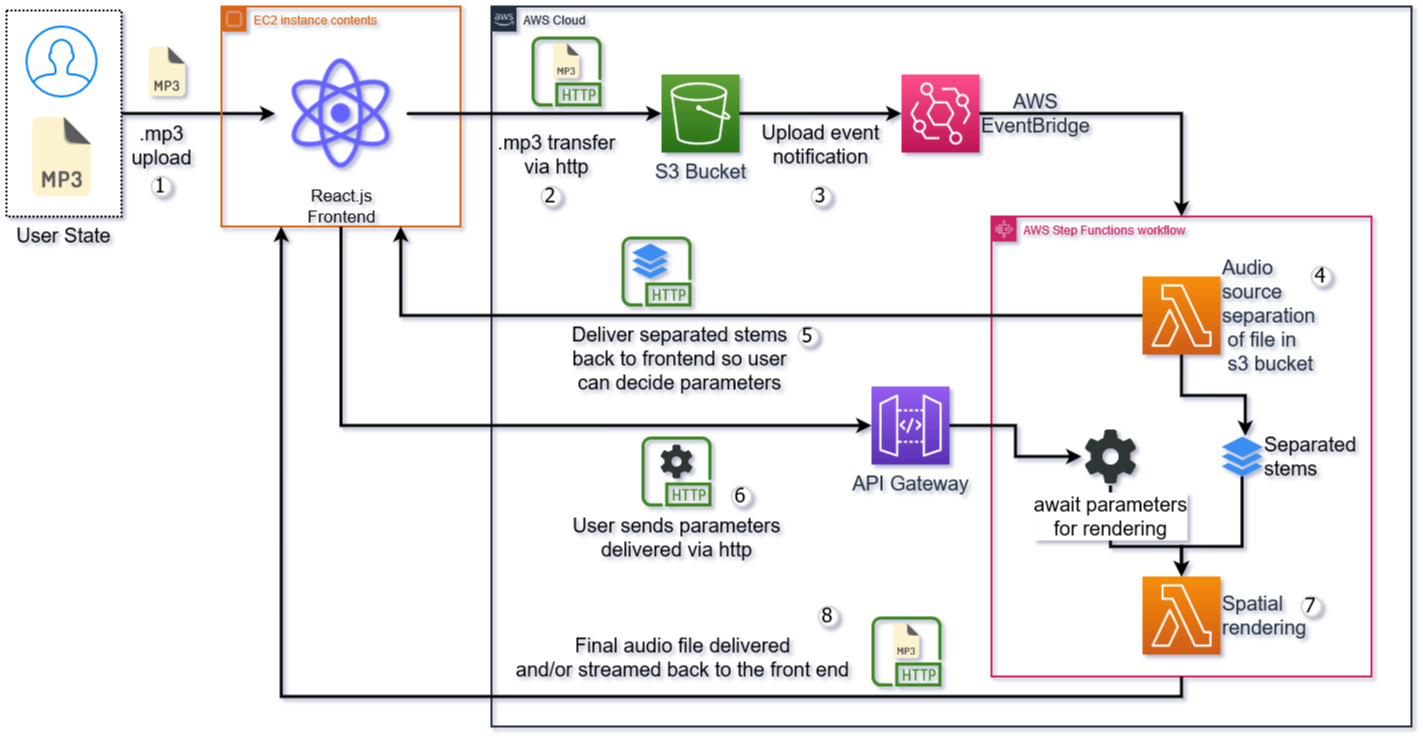
\includegraphics[width=\linewidth]{initial_architecture_diagram}
    \caption{Preliminary Design for Cloud Architecture}\label{fig:preliminary-design}
    \endminipage\hfill
\end{figure}

\subsection{Best Laid Plans}\label{subsec:best-laid-plans}

The product is designed for a wide range of users with varying knowledge of ~\gls{spatial_audio}.
In order to accommodate as many potential users as possible, a web-hosted~\gls{ui} is considered essential.
The user's primary mode of interaction with the service would be through a website
built using the~\gls{react} front-end library.
This library was chosen because of its ubiquity in modern web engineering; the depth of documentation available,
and existing familiarity with the framework.

The front-end was designed to make use of the~\gls{aws}~\gls{sdk} for~\gls{nodejs}.
This would allow the interface to initiate and interact with the audio processing pipeline hosted in~\gls{aws}.

Figure~\ref{fig:preliminary-design} also displays the two~\gls{aws-lambda} functions
that would comprise the backbone of the audio processing pipeline.
Furthermore,
these~\gls{aws-lambda} functions would be coordinated and executed using the~\gls{aws-step-function} service.
This service was highly desired for this purpose
since the processing pipeline would follow a series of discrete steps that require input from the user.
\glspl{aws-step-function} would be able to accommodate this easily.

The entire service was also initially intended
to be coordinated solely through the use of the internal messaging service:~\gls{aws-eventbridge}.
This service, in conjunction with~\gls{aws-api-gateway},
was intended to form the most of the communication between the back and front ends of the application.

\subsection{Refinement}\label{subsec:refinement}

As development progressed; it became apparent that there were issues with the initial design.

The first problems arose with the development of the~\gls{aws-lambda} functions that would be used to process the audio.
\gls{aws-lambda} functions
require a deployment package to be created
and then uploaded to~\gls{aws} in order for the function to have the resources it needs to run.
Unbeknownst to this author,
there is a limit of 50 MB on the size of the deployment packages that could be uploaded directly to~\gls{aws-lambda}.
Given that the 3D Tune-In Toolkit and the Spleeter source separation libraries have significant dependencies
that are more than 50 MB when zipped, a re-design needed to occur.

This issue was solved by making use of the~\gls{aws-ecr} service.
This service allows a developer to host and deploy~\glspl{container-image},
crucially, with a size limit of 75 GB allowed for each image uploaded to the registry.
Through the use of~\gls{docker} container images,
the code for the Lambda functions was bundled into deployment packages
that could be uploaded to an
\gls{aws-ecr} and then linked to a Lambda function
while staying well under the data limit offered by the container registry.
The Dockerfiles for the source separation and spatialisation lambda functions can be found in Appendix~\ref{subsec:lambda-function-dockerfiles}.
Note the installation of the AWS Lambda runtime environment for both Python in Listing~\ref{lst:source-sep-dockerfile} and C++ in Listing~\ref{lst:spatialisation-dockerfile}.

The next major revision to the architecture design came with the removal of the proposed~\gls{aws-api-gateway} interface.
Since the~\gls{aws-step-function} requires input from the user to execute,
the step function callback feature would be used to wait for an input message from the front end to the step function.
The most elegant solution for this problem was
to create a~\gls{aws-sqs} queue through which messages could be sent
and retrieved asynchronously without the risk of losing information through API communication failure.
This was implemented through the creation of a unique message queue per interaction with the product.
A unique identification key is created in the~\gls{react} interface, which is then used
to identify both the~\gls{aws-sqs} queue, and the resources uploaded and retrieved from the relevant~\gls{s3} buckets.
This key is not the same as a session key and would regenerate if the user refreshed the page to return to the start of the application.

With these changes, it became possible to define a final cloud architecture and workflow.

\subsection{Finalising the structure}\label{subsec:finalising-the-structure}

\begin{figure}[!htb]
    \minipage{\textwidth}
    \includesvg[width=\linewidth]{saas_architecture_2.0}
    \caption{Final cloud architecture diagram}\label{fig:final_design}
    \endminipage\hfill
\end{figure}

Figure~\ref{fig:final_design} depicts the final infrastructure design of the project.
The figure has been annotated with numbers to show the order in which data flows around the architecture.
In addition to the changes mentioned above, there are a few other notable changes that are evidenced in the figure.

\begin{itemize}
    \item The~\gls{aws-step-function} has been fleshed out with the discrete steps of the workflow orchestration.
    An Amazon States Language representation of the function can be found in Listing~\ref{lst:step-function-json}.
    \item There are three~\gls{s3} buckets to hold the artefacts from each stage of the process.
    \item The~\gls{react} frontend is now hosted in~\gls{amplify} instead of~\gls{ec2}; allowing for the implementation of~\gls{cicd} each time a commit is pushed to a branch in GitHub.
\end{itemize}

\subsection{A fresh coat of paint}\label{subsec:a-fresh-coat-of-paint}

